\begin{figure}[h]
%\begin{minipage}{0.49\textwidth}
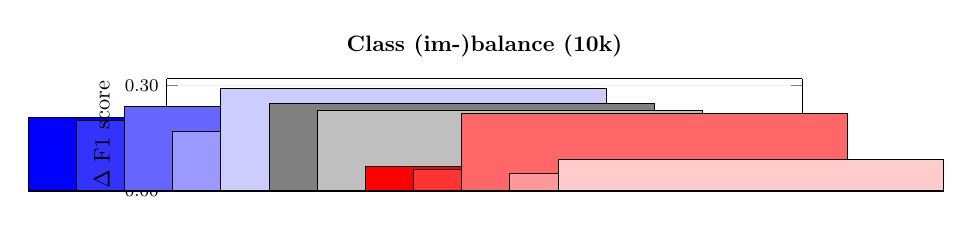
\begin{tikzpicture}[scale=0.95,every node/.style={scale=0.85}]
	\begin{axis}[
    		title=\textbf{Class (im-)balance (10k)},
		ylabel=$\Delta$ F1 score,
		scale only axis,
		clip=false,
		separate axis lines,
		xtick={1,2,3,4,5,6,7,8,9,10,11,12},
        	x tick style={draw=none},
        	xticklabels={Average,p-Means,SIF,GEM,Hier. pooling,BOREP,rand. BiLSTM,InferSent,Quick-Th.,sent2vec,BERT,LASER},
		xticklabels={,,},
		width=8.5cm,height=1.5cm,
		tick label style={font=\footnotesize},
		xticklabel style={rotate=90},
		ymajorgrids,
    		grid style={line width=.1pt, draw=gray!10},
		ymin=0,
		every axis plot/.append style={
          		ybar,
          		bar width=8.0,
          		bar shift=0.5pt,
			fill
		},
		scaled y ticks=false,
		y tick label style={
        		/pgf/number format/.cd,
            		fixed,
            		fixed zerofill,
            		precision=2,
        		/tikz/.cd
    		}
	]

		\addplot[draw=black,fill=blue] coordinates {(1,0.21)};
     	 	\addplot[draw=black,fill=blue!80] coordinates {(2,0.20)};
      		\addplot[draw=black,fill=blue!60] coordinates {(3,0.24)};
      		\addplot[draw=black,fill=blue!40] coordinates {(4,0.17)};
		\addplot[draw=black,fill=blue!20] coordinates {(5,0.29)};
     	 	\addplot[draw=black,fill=gray] coordinates {(6,0.25)};
      		\addplot[draw=black,fill=lightgray] coordinates {(7,0.23)};
      		\addplot[draw=black,fill=red] coordinates {(8,0.07)};
     	 	\addplot[draw=black,fill=red!80] coordinates {(9,0.06)};
      		\addplot[draw=black,fill=red!60] coordinates {(10,0.22)};
      		\addplot[draw=black,fill=red!40] coordinates {(11,0.05)};
		\addplot[draw=black,fill=red!20] coordinates {(12,0.09)};
	\end{axis}
\end{tikzpicture}
%\end{minipage}

%\begin{minipage}{0.49\textwidth}
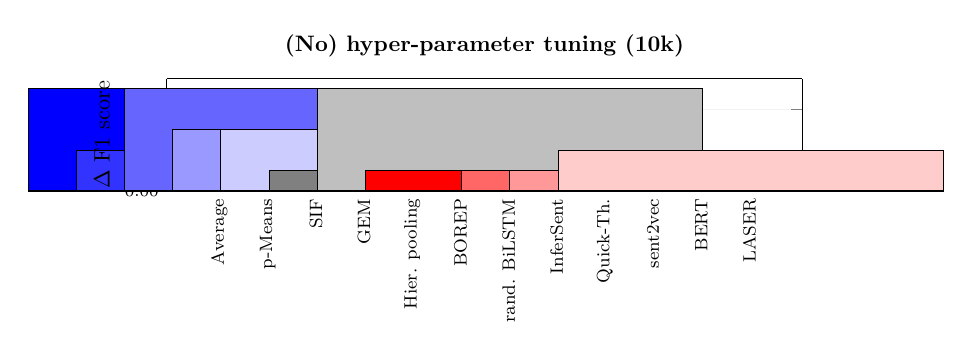
\begin{tikzpicture}[scale=0.95,every node/.style={scale=0.85}]
	\begin{axis}[
    		title=\textbf{(No) hyper-parameter tuning (10k)},
		ylabel=$\Delta$ F1 score,
		scale only axis,
		clip=false,
		separate axis lines,
		xtick={1,2,3,4,5,6,7,8,9,10,11,12},
        	x tick style={draw=none},
        	xticklabels={Average,p-Means,SIF,GEM,Hier. pooling,BOREP,rand. BiLSTM,InferSent,Quick-Th.,sent2vec,BERT,LASER},
		width=8.5cm,height=1.5cm,
		tick label style={font=\footnotesize},
		xticklabel style={rotate=90},
		ymajorgrids,
    		grid style={line width=.1pt, draw=gray!10},
		ymin=0,
		every axis plot/.append style={
          		ybar,
          		bar width=8.0,
          		bar shift=0.5pt,
			fill
		},
		scaled y ticks=false,
		y tick label style={
        		/pgf/number format/.cd,
            		fixed,
            		fixed zerofill,
            		precision=2,
        		/tikz/.cd
    		}
	]

		\addplot[draw=black,fill=blue] coordinates {(1,0.05)};
     	 	\addplot[draw=black,fill=blue!80] coordinates {(2,0.02)};
      		\addplot[draw=black,fill=blue!60] coordinates {(3,0.05)};
      		\addplot[draw=black,fill=blue!40] coordinates {(4,0.03)};
		\addplot[draw=black,fill=blue!20] coordinates {(5,0.03)};
     	 	\addplot[draw=black,fill=gray] coordinates {(6,0.01)};
      		\addplot[draw=black,fill=lightgray] coordinates {(7,0.05)};
      		\addplot[draw=black,fill=red] coordinates {(8,0.01)};
     	 	\addplot[draw=black,fill=red!80] coordinates {(9,0.00)};
      		\addplot[draw=black,fill=red!60] coordinates {(10,0.01)};
      		\addplot[draw=black,fill=red!40] coordinates {(11,0.01)};
		\addplot[draw=black,fill=red!20] coordinates {(12,0.02)};
	\end{axis}
\end{tikzpicture}
%\end{minipage}
%
%\vspace*{4mm}
%\begin{minipage}{0.49\textwidth}
%\begin{tikzpicture}[scale=0.75,every node/.style={scale=0.85}]
%	\begin{axis}[
%    		title=\textbf{NN $\leftrightarrow$ NN\_H (10k)},
%		ylabel=$\Delta$ F1 score,
%		scale only axis,
%		clip=false,
%		separate axis lines,
%		xtick={1,2,3,4,5,6,7,8,9,10,11,12},
%        	x tick style={draw=none},
%        	xticklabels={Average,p-Means,SIF,GEM,Hier. pooling,BOREP,rand. BiLSTM,InferSent,Quick-Th.,sent2vec,BERT,LASER},
%		width=6.5cm,height=2cm,
%		tick label style={font=\footnotesize},
%		xticklabel style={rotate=90},
%		ymajorgrids,
%    		grid style={line width=.1pt, draw=gray!10},
%		every axis plot/.append style={
%          		ybar,
%          		bar width=8.0,
%          		bar shift=0.5pt,
%			fill
%		},
%		scaled y ticks=false,
%		y tick label style={
%        		/pgf/number format/.cd,
%            		fixed,
%            		fixed zerofill,
%            		precision=2,
%        		/tikz/.cd
%    		}
%	]
%
%		\addplot[draw=black,fill=blue] coordinates {(1,-0.04)};
%     	 	\addplot[draw=black,fill=blue!80] coordinates {(2,-0.03)};
%      		\addplot[draw=black,fill=blue!60] coordinates {(3,-0.01)};
%      		\addplot[draw=black,fill=blue!40] coordinates {(4,0.01)};
%		\addplot[draw=black,fill=blue!20] coordinates {(5,-0.04)};
%     	 	\addplot[draw=black,fill=gray] coordinates {(6,-0.01)};
%      		\addplot[draw=black,fill=lightgray] coordinates {(7,-0.08)};
%      		\addplot[draw=black,fill=red] coordinates {(8,-0.02)};
%     	 	\addplot[draw=black,fill=red!80] coordinates {(9,-0.02)};
%      		\addplot[draw=black,fill=red!60] coordinates {(10,0.00)};
%      		\addplot[draw=black,fill=red!40] coordinates {(11,0.02)};
%		\addplot[draw=black,fill=red!20] coordinates {(12,-0.08)};
%	\end{axis}
%\end{tikzpicture}
%\end{minipage}
%\hfill
%\begin{minipage}{0.49\textwidth}
%\begin{tikzpicture}[scale=0.75,every node/.style={scale=0.85}]
%	\begin{axis}[
%    		title=\textbf{Size (10k $\leftrightarrow$ 30k)},
%		scale only axis,
%		clip=false,
%		separate axis lines,
%		xtick={1,2,3,4,5,6,7,8,9,10,11,12},
%        	x tick style={draw=none},
%        	xticklabels={Average,p-Means,SIF,GEM,Hier. pooling,BOREP,rand. BiLSTM,InferSent,Quick-Th.,sent2vec,BERT,LASER},
%		width=6.5cm,height=2cm,
%		tick label style={font=\footnotesize},
%		xticklabel style={rotate=90},
%		ymajorgrids,
%    		grid style={line width=.1pt, draw=gray!10},
%		ymin=0,
%		every axis plot/.append style={
%          		ybar,
%          		bar width=8.0,
%          		bar shift=0.5pt,
%			fill
%		},
%		scaled y ticks=false,
%		y tick label style={
%        		/pgf/number format/.cd,
%            		fixed,
%            		fixed zerofill,
%            		precision=2,
%        		/tikz/.cd
%    		}
%	]
%
%		\addplot[draw=black,fill=blue] coordinates {(1,0.09)};
%     	 	\addplot[draw=black,fill=blue!80] coordinates {(2,0.08)};
%      		\addplot[draw=black,fill=blue!60] coordinates {(3,0.07)};
%      		\addplot[draw=black,fill=blue!40] coordinates {(4,0.01)};
%		\addplot[draw=black,fill=blue!20] coordinates {(5,0.08)};
%     	 	\addplot[draw=black,fill=gray] coordinates {(6,0.08)};
%      		\addplot[draw=black,fill=lightgray] coordinates {(7,0.13)};
%      		\addplot[draw=black,fill=red] coordinates {(8,0.02)};
%     	 	\addplot[draw=black,fill=red!80] coordinates {(9,0.05)};
%      		\addplot[draw=black,fill=red!60] coordinates {(10,0.01)};
%      		\addplot[draw=black,fill=red!40] coordinates {(11,0.04)};
%		\addplot[draw=black,fill=red!20] coordinates {(12,0.03)};
%	\end{axis}
%\end{tikzpicture}
%\end{minipage}
\end{figure}